\chapter{対話雰囲気推定モデルの構築\label{sec:develop_estimation_model}}
\thispagestyle{plain}

本研究では,機械学習によって通話中の音声から対話雰囲気を推定する.
本研究で構築する対話雰囲気推定モデルは,対話データから抽出した特徴量を入力値とし,第\ref{node:estimated_atmosphere}項で述べた各雰囲気について肯定,否定の2値での分類結果を出力値とする.
豊田らは二者対話を対象に発話時間特徴を特徴量とする機械学習を用いた対話雰囲気推定を行なっている\cite{Toyota}.
豊田らの構築したモデルは「盛り上がり」「まじめさ」「噛み合い」「明るさ」「親密さ」「対等さ」の6つの雰囲気を推定対象としており,それぞれ肯定,否定の2値で分類している.
特に「盛り上がり」「まじめさ」「親密さ」の推定においては全体正答率が0.8を超える高い値を示していることから,本研究でもこの手法に基づいて対話雰囲気推定モデルの構築を行う.
本章では,本研究における対話雰囲気推定モデルの構築手順について述べる.

\section{対話データの収集とラベル付け}

学習データを構築するために対話データの収集を行う.
豊田らは対話データとして音声コーパス\cite{PASD}を採用している.
一方で,本研究では実際に開催された作業通話の録音データを採用する.
これは一般的な対話と作業通話中の対話はそれぞれ性質が異なるためである.
例えば,一般的な対話では沈黙は気まずく回避される傾向があるが,作業通話における沈黙は作業に集中していることの現れであり許容される傾向がある.
加えて,作業通話中の対話においては突発的な話題の変化が起こりやすく,独り言が行き交うことが多いなどの特徴がある.
このような作業通話中の対話の独特な性質が,対話雰囲気の形成に影響を与えていると十分に考えられることから,本研究では実際の作業通話の音声を学習に用いる.

対話データの収集とラベル付けの手順について述べる.
まず,対話データとして1 〜 4名の話者からなる計6時間弱の作業通話音声の録音を行う.
次に全ての音声を10 〜 120秒程度の対話になるように切り出す.
続いて,それぞれのデータに対して第\ref{node:estimated_atmosphere}項で述べた各雰囲気(「盛り上がり」,「真面目さ」,「明るさ」,「くつろぎ」)について主観で肯定か否定のラベル付けを行う.
ここで付与するラベルはのちの学習での教師ラベルとなる.
以上の手順により本研究では,計130対話を抽出しラベル付けされた対話データとした.

\section{発話状態集合の抽出}

特徴量の抽出を行うために,対話データから発話状態集合の抽出を行う.
発話状態集合とは,対話データにおける話者ごとの発話時間を発話状態ごとに記録した集合のことを指す.
豊田らの手法では,一つの対話データについて各話者の単独発話集合と二者の同時発話集合を抽出している.
この手法は二者の対話でのみ有効な抽出方法である.
しかし,本研究の手法における対象話者数は2 〜 4名であるため,異なる手法を用いて発話状態集合を抽出する.

はじめに,豊田らの手法は1名の話者のみが発話している状態を単独発話状態としてその集合を抽出しているが,本研究では他の話者の発話に依存せず話者ごとに発話している状態を発話集合として抽出する.
図\ref{fig:speaker_split}を例に述べる.
図\ref{fig:speaker_split}は対話データの一部を例として掲載しており,横軸が時間の流れを表している.
また,縦軸の各話者と同じ高さで引かれている線はそれぞれの話者が発話していることを表している.
図\ref{fig:speaker_split}において豊田らの手法の場合,話者$A$における単独発話集合は$\{3, 4, 3, 3, ...\}$となる.
一方本研究の場合,話者$A$における発話集合は$\{3, 5, 3, 3, ...\}$となる.

\begin{figure}
    \centering
    \fbox{
        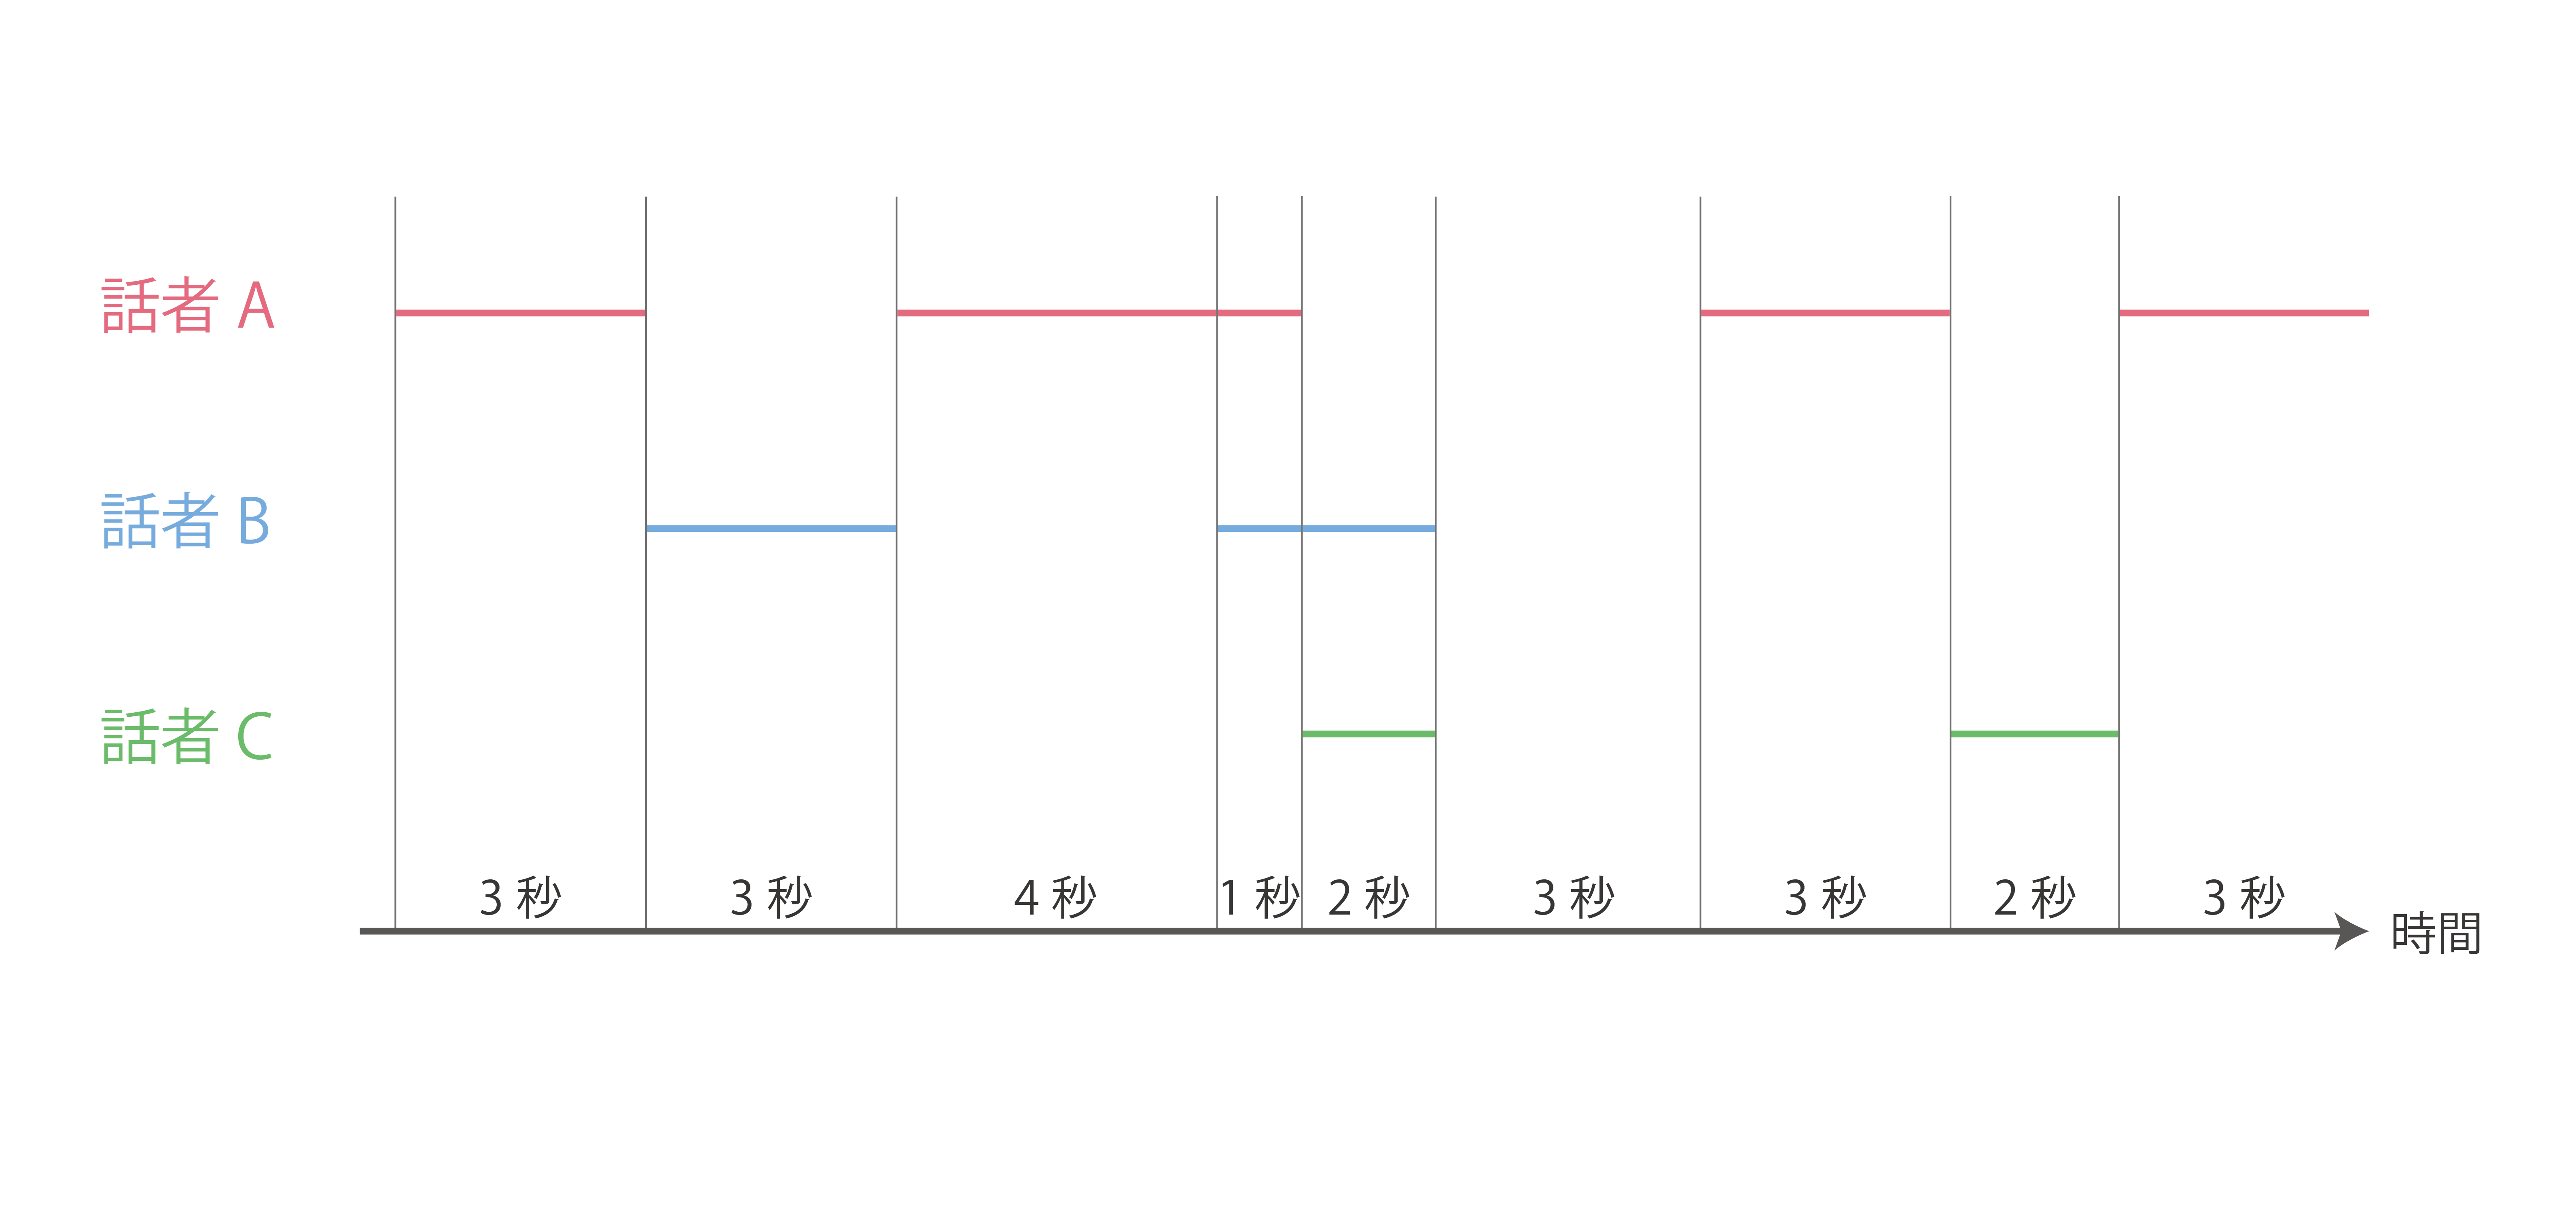
\includegraphics[width=0.7\textwidth]{figs/speaker_split.png}
    }
    \caption{対話データにおける発話の例}
    \label{fig:speaker_split}
\end{figure}

次に,豊田らの手法は二名の話者が同時に発話している状態を同時発話状態としてその集合を対話データにつき一つ抽出しているが,本研究では話者ごとに同時発話集合を抽出する.
図\ref{fig:speaker_split}において豊田らの手法の場合,同時発話集合は$\{1, 2, ...\}$となる.
一方本研究の場合,話者ごとに抽出するため話者$A$の同時発話集合は$\{1, ...\}$,話者$B$の同時発話集合は$\{1, 2, ...\}$,話者$C$の同時発話集合は$\{2, ...\}$となる.

以上が豊田らの手法で抽出した発話状態集合との比較である.
加えて本研究では,一つの対話データ全体としての傾向が対話雰囲気の形成に影響を与えていると仮定し,新たに三つの発話状態を定義しそれらの集合を抽出した.
一つ目は非発話状態である.
非発話状態は対話において一人も発話していない状態である.
非発話状態の集合である非発話集合は図\ref{fig:speaker_split}の場合,$\{3, ...\}$となる.
二つ目は全発話状態である.
全発話状態は全話者の発話状態を集約した発話状態である.
全発話状態の集合である全発話集合は図\ref{fig:speaker_split}の場合,$\{3, 5, 3, 3, 3, 3, 2, 2, ...\}$となる.
三つ目は全状態である.
全状態は全発話集合へ非発話状態を加えた状態である.
全状態の集合である全集合は図\ref{fig:speaker_split}の場合,$\{3, 5, 3, 3, 3, 3, 2, 2, 3 ...\}$となる.

以降,対話$d$におけて話者数は$n$,任意の発話状態集合は$S^d$と表現し,その集合における$i$番目の要素は$S^di$と表現する.
加えて,話者$x$についての発話集合は$S^d_{stx}$,同時発話集合は$S^d_{ssx}$と表現する.
また,同様に対話$d$に対する非発話集合は$S^d_{ns}$,全発話集合は$S^d_{us}$,全集合は$S^d_{as}$と表現する.

\section{特徴量の抽出}

抽出した発話状態集合から特徴量の抽出を行う.
豊田らは各集合に対する統計量とその統計量を比較した値(以下,「比較量」)を算出し特徴量としている.
本研究でも統計量と比較量を特徴量とするが,具体的に算出する値は異なる.

\subsection{統計量の抽出}

本研究で特徴量として採用する統計量とそれらの算出式を表\ref{tab:statistics_and_formulas}に示す.
本研究では,統計量としてそれぞれの集合に対する合計値,平均値,標準偏差,最大値,要素数,占有率を算出する.
それぞれの統計量の採用理由について述べる.
はじめに,合計値と平均値,要素数,占有率を計測することで話者の会話への積極性や興味の強さが対話雰囲気の形成に与える影響を測定するために採用した.
次に,標準偏差は話者間の発話の偏りが対話雰囲気の形成に与える影響を測定するために採用した.
最大値は対話における発話時間の値域が対話雰囲気の形成に与える影響を測定するために採用した.

\begingroup
\renewcommand{\arraystretch}{1.5}
\begin{table}[t]
    \caption{特徴量として採用する統計量と算出式}
    \centering
    \begin{tabular}{ll}
        \hline
        統計量 & 算出式 \\
        \hline\hline
        合計値 & $sum(S^d) = \sum_{i=1}^n S^di$ \\
        \hline
        平均値 & $mean(S^d) = \frac{sum(S^d)}{n}$ \\
        \hline
        標準偏差 & $std(S^d) = \sqrt{\frac{1}{n}\sum_{i=1}^n (S^di - mean(S^d))^2}$ \\
        \hline
        最大値 & $max(S^d) = \{r\in{S^d} | r \geq \forall{a}\in{S^d} \}$ \\
        \hline
        要素数  & $size(S^d) = |S^d|$ \\
        \hline
        占有率  & $share(S^d) = \frac{sum(S^d)}{sum(S^d_{as})}$ \\
        \hline
    \end{tabular}
    \label{tab:statistics_and_formulas}
\end{table}
\endgroup

\subsection{比較量の抽出}

統計量をもとに比較量を算出する.
本研究における二つの発話状態集合の比較量は,発話状態集合の各統計量について発話合計時間が短い方を長い方で除算することで算出する.
よって比較を行う発話状態集合両者に欠損値が存在しない場合は,一回の比較で6つの比較量が得られる.
本研究は比較量として話者間発話比較,話者間同時発話比較,他話者比較,話者内発話比較を算出する.

はじめに,話者間発話比較は,対話$d$における任意の話者二名の発話状態を比較した値である.
話者間発話比較を求めることで,話者間の発話時間や発話頻度の比較を行うことができる.
これによって,対話における話者間のコミュニケーション量の違いが対話雰囲気の形成に与える影響を測定することができることから話者間発話比較を採用した.

次に,話者間同時発話比較は,対話$d$における任意の話者二名の同時発話状態を比較した値である.
話者間の発話量の比較について,二者の対話における同時発話状態の発生回数や占有率などの統計量が「盛り上がり」や「真面目さ」の対話雰囲気に影響を与えることが示唆されている\cite{Ito}\cite{Toyota}.
本研究では,同時発話集合を話者ごとに抽出しているため同様に同時発話状態の比較が対話雰囲気の推定に有効であると考え話者間同時発話比較を採用した.

続いて,他話者比較は,対話$d$における任意の話者一名と,その話者以外の話者の発話集合を結合させた集合を比較した値である.
他話者比較を求めることで,特定の話者だけでなく対話全体の中での発話時間や発話頻度を求め対象話者が聞き手であるか,話し手であるかを推定できる.
これにより,聞き手(話し手)の発話量が対話雰囲気に与える影響を測定できることから他話者比較を採用した.

話者内発話比較は,対話$d$における任意の話者一名の発話状態と同時発話状態を比較した値である.
話者内発話比較を求めることで,対話において一人の話者が一方的に発言を続けているかを推定することができる.
これにより,話者が他話者の発言をどの程度受け入れているかを測定できることから話者内発話比較を採用した.

% 生成した発話集合から特徴量の抽出を行う.
% 豊田らは各集合に対する統計量とその統計量を比較した値(以下,「比較量」)を算出し特徴量としている.
% 本研究でも統計量と比較量を特徴量とするが,具体的な算出式は異なる.
% まず,それぞれの集合に対して平均値,標準偏差,最大値,要素数を算出する.
% 加えて,全集合以外の集合に対して占有率を算出し,全発話集合と全集合に対して合計値を算出する.
% 以上全てを特徴量として用いる.その後それぞれの特徴量の比較を行いそれらも特徴量とする.
% これは各話者単体や全体に着目するだけでなく,各話者間や各話者と全体の比較を行うことで一部の雰囲気の推定に有効と仮説を立てたためである.
% 例えば,話者間に極端な発話時間・回数の差があるデータと,話者間の発話時間・回数に差があまりないデータが存在した場合,前者に比べ後者は議論が活発化しており真面目な雰囲気なことが多いのではないかと推測できる.
% 比較量を求める際に比較する値はそれぞれの集合の同じ統計量である.
% 例えば,発話時間が最も長いA話者の単独発話集合とB話者の単独発話集合を平均値で比較する場合は,A話者の単独発話集合の平均値をB話者の単独発話集合の平均値で除算することで算出する.
% 比較の際には話者間発話比較,話者間同時発話比較,話者内発話・非発話比較,全発話・発話比較を行う.
% 結果として各対話データにつき210個の特徴量が算出される.
% ただし,210個というのは最大値であり実際に算出される特徴量数は話者数により異なる.
% そのため,前処理として学習データ間に利用特徴量数の差があった場合は,話者数に合わせ特徴量や学習データの削除を行い新しい学習データとする.

\section{学習と特徴量選択}

算出された特徴量を用いて学習を行う.
本研究の学習の方法は,対象とする雰囲気や話者数が豊田らと異なるため,一部独自の手法を採用する.
本研究では,雰囲気,話者数ごとに対話雰囲気推定モデルの構築を行う.
これは各雰囲気や話者数によって有効な特徴量が異なるという仮説に基づいているためである.
本研究で学習を行う際には対象雰囲気,対象話者数,学習アルゴリズムの設定を行う.
本研究の対象雰囲気は「盛り上がり」,「真面目さ」,「明るさ」,「くつろぎ」の4つから選択する.
対象話者数は2〜4名から選択する.
学習モデルにはどの学習モデルが本研究の学習において有効であるか比較を行うため,Linear SVC,k近傍法,SVC,Naïve Bayesの4つを採用する.

また,本研究では豊田らの手法にならい,遺伝的アルゴリズム(以下,「GA」)を用いた特徴量選択を行う.
特徴量選択を行うことで精度の向上や安定化が期待できる.
具体的な手法も豊田らの手法を参考にする.
GAでは特徴量数と同じ長さのビット列からなる染色体を生成し,各特徴量の利用有無を1:有効,0:無効で表現する.
GAにおける設定の一部を表\ref{tab:ga_setting}に記載する.
表中の評価における「選択特徴量数と正答率の重み付け和による評価」は以下の式によって算出する.
式中の$W$は正答率と選択特徴量数の重み付けを表現しており,$[0, 1]$の値をとる.

\begin{table}[t]
    \caption{遺伝的アルゴリズムの設定}
    \centering
    \begin{tabular}{ll}
        \hline
        設定項目 & 範囲・候補 \\
        \hline\hline
        評価 & 正答率による評価 \\
        & 選択特徴量数と正答率の重み付け和による評価 \\
        \hline
        検証 & 交差検証の有無 \\
        \hline
        突然変異確率 & 突然変異確率 \\
        \hline
        交叉  & 一様交叉 \\
        & 二点交叉 \\
        \hline
        集団の大きさ  & 100 \\
        \hline
        エリート染色体選択数  & 20 \\
        \hline
        世代数  & 250 \\
        \hline
    \end{tabular}
    \label{tab:ga_setting}
\end{table}

\begin{equation}
    評価値 = \frac{正答数}{検証データ数} W + (1 - \frac{選択特徴量数}{全特徴量数}) (1 - W)
\end{equation}
